%ResultsAndDiscussion

\subsection{Goals}
First, let's have a look at what our goals were. We planned to have a look at the pedestrian flux, how it can be improved and jammings be avoided. We furthermore wanted to have a closer look to what happens during rush-hours and in a situation when much more people are moving in one direction than in the other.\\
On the agent-based side of our model, we wanted to analyze the influence of aggressive fast people in a rush, slowly moving obstacles (eg. mothers with baby buggies) and the influence of drunkard (more or less randomized walking) on the pedestrian flux.\\
If everything went well, we also wanted to implement a static obstacle and see what happens. As a reminder before the discussion of the results, our fundamental research questions were:
\begin{itemize}
\item How does the simulation behave in the following situations: rush hour, with obstacle, with very slow/fast agents, random path agent (drunkard)? Does it run smoothly or will ther be jams?
\item How will our implementation of a rudimentary kind of "thinking ahead" affect the simulation? Will it work good or bad? Can we compare it to other implementations?
\item Are there any group dynamics evolving as lane or group formation?
\end{itemize}

\subsection{General achievements}
As soon as we started programming we realized there was a major point of importance about this work we all were aware of, but had forgot to put it in the project proposal. We all did not want to start with an already known program or existing algorithms, but build something "new" on our own. So we started off creating our logic function that would allow the agents to avoid crashing into other agents and not working with repulsive forces as for example Helbing in \ref{helbing} did.\\
Quite proudly, we can now say we managed to do this. Our idea of the agents "thinking ahead" by consulting where other agents are and not just being pushed around by repulsive forces worked.\\
We now are able to play with lots of input variables, the most important being number of agents entering the corridor per time and the agents' characteristics as size, speed and lots more.\\
A nice thing we built but did not originally plan to is that we planned to and did research on the situation as explained earlier in the long, narrow corridor in Zurich main station. But in our simulation, one can also change dimensions as length and shape of the walls easily as well as inserting obstacles.\\

\noi We therefore decided first of all to make sure that the model works and what its operating parameters are. This meant that we had to drop a lot of our former goals because we did not want to carry on with a faulty model. Therefore we have included some results that were not included in our first questions we set out to answer in the beginning.\\
On the downside of this, we dropped the investigation into the behaviour of the pedestrian flux when exposed to aggressive, slow or random people. Even though these situations were not simulated, the functionality to introduce them without much work was implemented into the model as they were considered when we built our model.

\subsection{Results from the simulation series}
\subsubsection{Influence of different pedestrian flux densities}
% Influence of different pedestrian flux densities

\noi For this experiment we monitored the total agents count as an indicator for jams. This number was then scaled by the combined flux densities to give comparable results which can be found in figure \ref{fig:AAllAveragesScaled}.\\
\begin{figure}[h!]
	\centering
		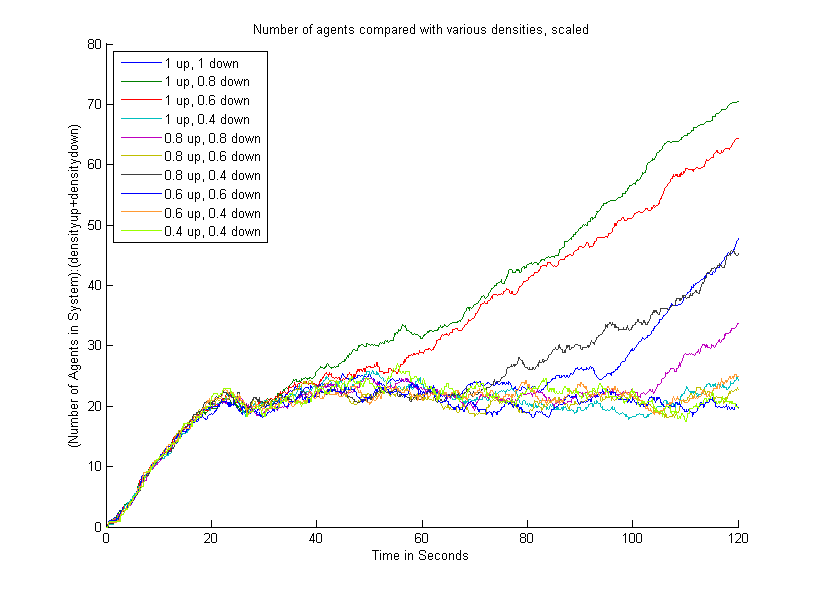
\includegraphics[width=0.80\textwidth]{pictures/AAllAveragesScaled.png}
	\caption{The scaled total number of agents in the system for various combinations of flux densities with respect to time. The used flux densities are given in the graph legend. As soon as the total number of agents runs away, a jam has formed. The mean over three simulations with different seeds was taken for each case. As expected high flux densities caused massive jams.}
	\label{fig:AAllAveragesScaled}
\end{figure}

\noi With the highest flux densities used in the simulations, the jam formation was very fast. It is interesting that 0.6/0.6, 0.8/0.4 and 0.8/0.8 also caused jams within the observed time frame, specially since 1/0.4 didn't jam.\\
Our model seems not to be able to cope well with that many people. There should be more simulations with different seeds to get a better statistic.\\

\begin{figure}[h!]
	\centering
		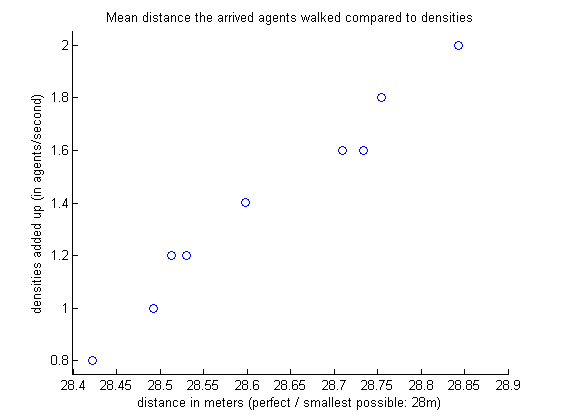
\includegraphics[width=0.49\textwidth]{pictures/AMeanDistancesCompared.png}
		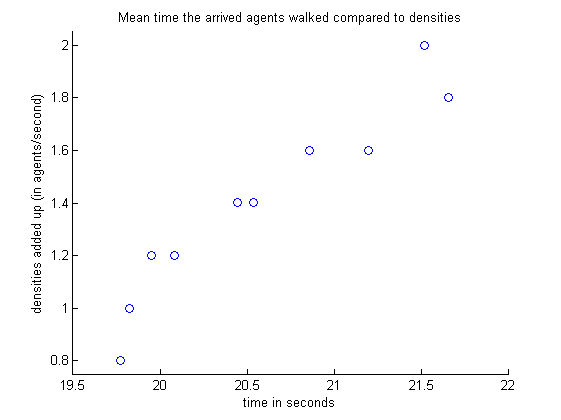
\includegraphics[width=0.49\textwidth]{pictures/AMeanTimeCompared.png}
	\caption{Graphs of the mean covered distance and mean time spent during the simulation for all agents who reached their destruction line compared with the combined flux densities used. As expected, for high flux densities the agents have to cover longer distances and spend more time as they have to avoid colliding with other agents.}
	\label{fig:ACompared}
\end{figure}

\noi Given in figure \ref{fig:ACompared} are the mean covered distance and mean time spent during the simulation for all agents who reached their destruction line compared with the combined flux densities used. As would be expected, the agents had to cover a longer distance and spend more time in the simulation as they had to avoid collisions with other agents.\\
These variables were monitored to analyze whether they give a good description of the model and to ensure that we got results that run within the same expectations as in reality. But as they only take the values of those agents that have left the simulation, they may have a decreased significance when jams occur and are not at all able to tell whether a jam has occured or not.




\subsubsection{Influence of overtaking or lane formation on the success of the model}
% Influence of overtaking or lane formation on the success of the model

\begin{figure}[h!]
	\centering
		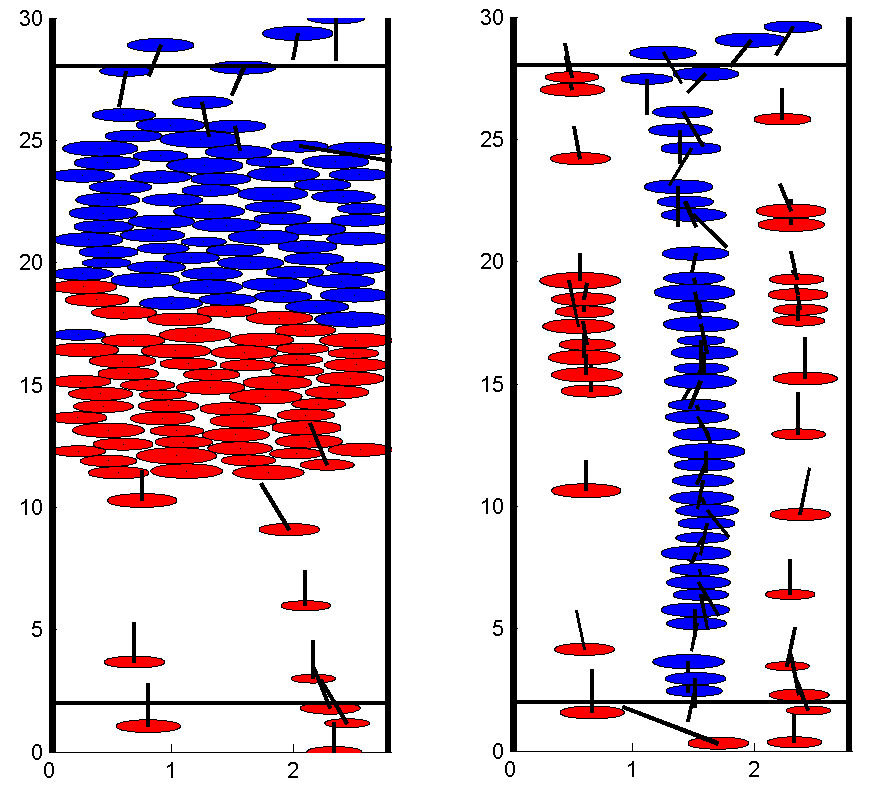
\includegraphics[width=0.8\textwidth]{pictures/ex2picture.png}
	\caption{Exemplary pictures of our simulation after a simulation time of 120 seconds. The right one was run with a \texttt{DISPERSIONFACTOR} of 1 while the left picture has one of 0.1. The jaming to the left and the lane formation to the right can be seen.}
	\label{fig:ex2picture}
\end{figure}

\noi Some examples of how our simulation did look like after a simulation time of 120 second are given in \ref{fig:ex2picture}.\\

\noi In figure \ref{fig:AAllInOne} all collected data is consensed into one graph which was visualized in two ways. Another representation of the same data is given in the appendix in figure \ref{fig:ADistanceSeedsFactors} (page \pageref{fig:ADistanceSeedsFactors}). They correlate the average distance covered per agent per iteration step with the simulation time. There were two expectations: As soon as a jam starts to form, this variable should decrease quite fast. An lane formation should be detectable as most agents will not be able to walk with their maximum speed so the average distance per agent per timestep should be significantly below the mean value given by $\bar{d} = \Delta t \cdot \bar{v}$, the product of \texttt{DELTAT} with \texttt{MEANSPEED}.\\

\begin{figure}[h!]
	\centering
		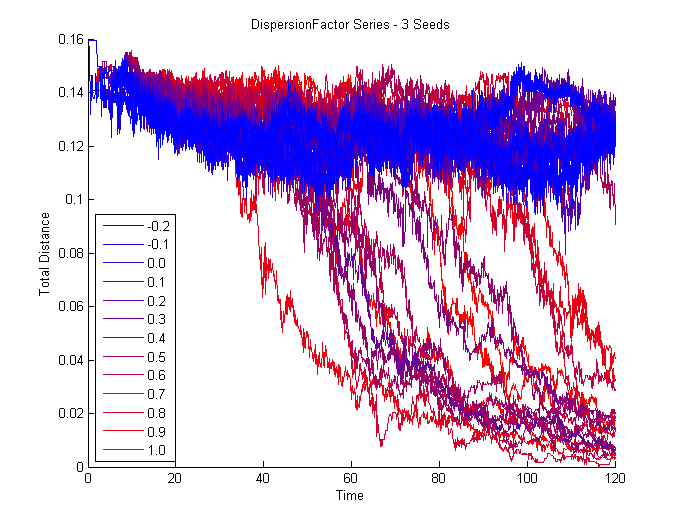
\includegraphics[width=0.49\textwidth]{pictures/AAllInOneColorsBlue.png}
		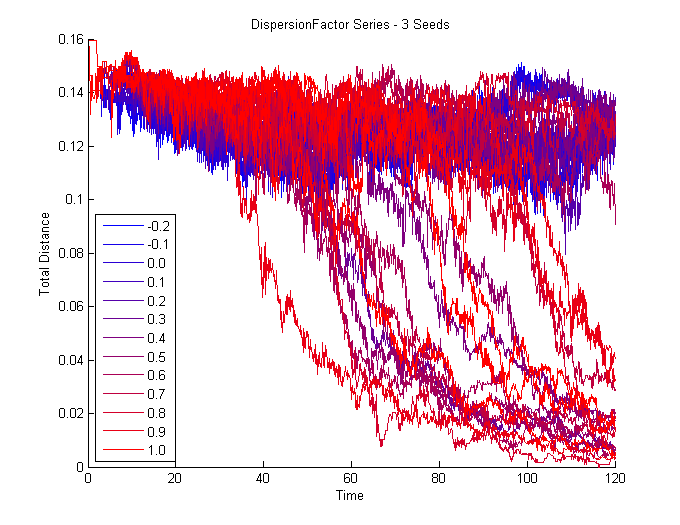
\includegraphics[width=0.49\textwidth]{pictures/AAllInOneColorsRed.png}
	\caption{Graph of the average covered distance per agent present in the simulation per step as a function of time. The more blueish the color is, the stronger was the agents tendency to form lanes while the more reddish the color is, the stronger was the agents tendency to try to overtake slow agents. In the left graph the more blue lines are highlighted while in the right graph the more red lines are highlighted. Although the red lines representing "greedy" agents cope well at the very start, the usually lead to a jam very quickly.}
	\label{fig:AAllInOne}
\end{figure}

\noi Given the two graphs, it is striking that the majority of the simulations represented by reddish lines representing high values of \texttt{DISPERSIONFACTOR} fail during the observed time frame. At rare occasion though the simulation was successful even with a relatively high \texttt{DISPERSIONFACTOR}.\\
On the other side, there was always lane formation for a \texttt{DISPERSIONFACTOR} below 0.4, represented by the more blueish lines which ultimately resultet mostly in successful simulations without jamming.\\
The lane formation can be seen quite clearly in the graphs given in figure \ref{fig:AAllInOne}. The reddish lines try to keep the mean distance at almost all cost, this is visible in the initial height of the reddish lines. In contrast, the blueish lines quickly fall down by about 0.02 meters per agent per iteration step which is a precise indication of lane formation. But in the long run, the best reddish line performed about equally well as most blueish lanes, indicating that in crowded situations like this, cooperation between agents in the form of line formation is not worse in peformance as the best egoistic approach but succeeds way more often.\\

\noi It seems that the forced lane formation was a successful way to resolve the problem of jaming. It also highlights the importance of cooperation and the sensitivity of our model towards this parameter.

\label{ex2}

\subsubsection{Influence of the radius of sight of an agent}
% Influence of the radius of sight of an agent

\noi The constant variable INFLUENCESPHERE determines the radius of the semi-circle in which the agent considers other agents around him. With flux densities of 1.0 each and a DISPERSIONFACTOR of 0.7, the INFLUENCESPHERE was tested using the values 1.5, 2.0, 2.5 and 3.0 (in meters). This was done for three seeds each, 51, 77 and 151. All simulations were run for 120 seconds.

\begin{figure}[h!]
	\centering
		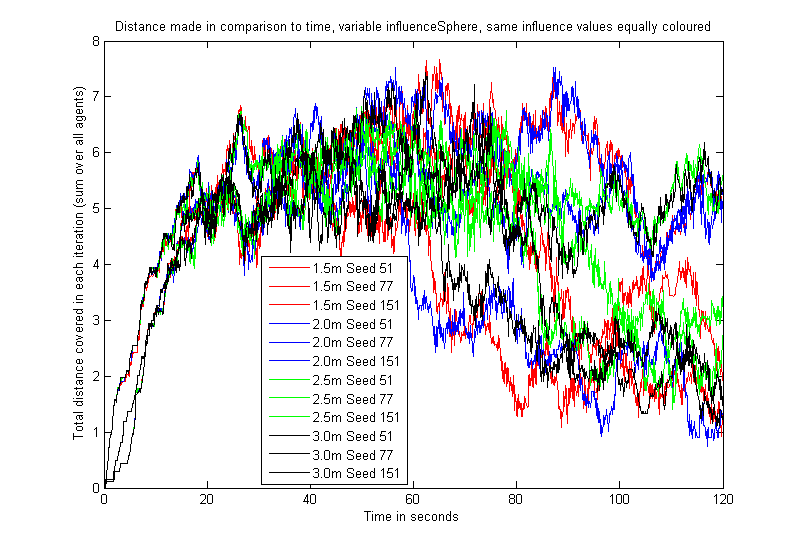
\includegraphics[width=0.80\textwidth]{../../code/sim/Influence/ATotalDistanceInfluencesColoured.png}
	\caption{This plot shows the total distance covered by all agents in the system for different influence sphere radii and seeds in dependence of the simulation time. This distance decreases rapidly when a jam starts. To show the total distance's dependence on the influence sphere radius, each seed to a certain radius was coloured equally. Only these radii were varied in these simulations. One can see here that there is no clear dependence of the radii to the total distance as for every radius except 1.5m there are seeds that work and seeds that don't, which means they had jams.}
	\label{fig:InfluencesColoured}
\end{figure}

First of all, the dependency between the influence sphere's radius and the total distance walked by all agents has to be evaluated. As shown in figure \ref{fig:InfluencesColoured}, neither dependencies nor tendencies can be seen clearly, as of every radius, some seeds worked well where other simulations for the same seed jammed.

\begin{figure}[h!]
	\centering
		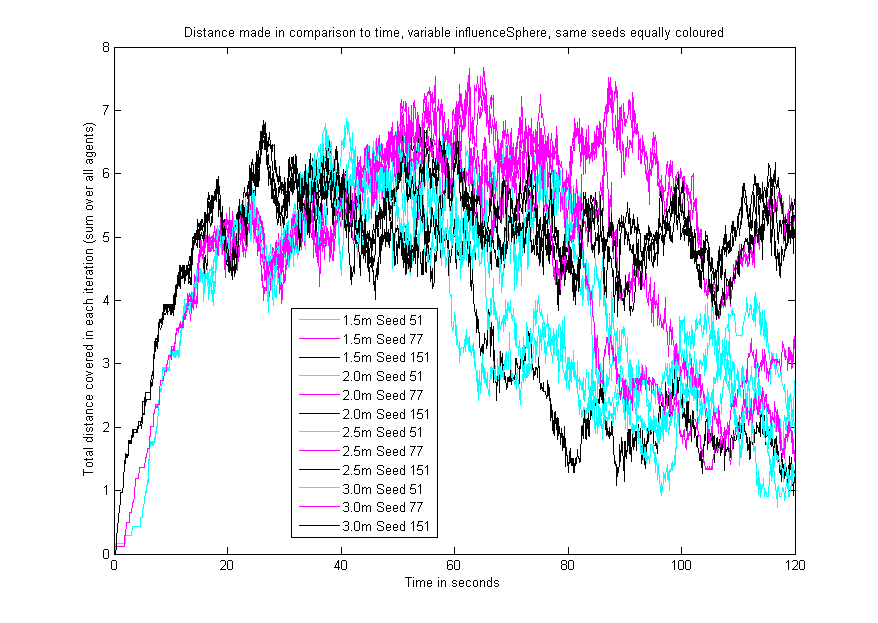
\includegraphics[width=0.80\textwidth]{../../code/sim/Width/ATotalDistanceSeedsColoured.png}
	\caption{This plot shows the total distance covered by all agents in the system for different influence sphere radii and seeds in dependence of the simulation time. This distance decreases rapidly when a jam starts. To show the total distance's dependence on the seed, each radius to a certain seed was coloured equally. Only these radii were varied in these simulations. One can see here that whether a simulation jams or not seems to depend on the seed, as the seed 51 simulations all jammed independent of the radius, and for the other two seeds, there was only one radius that was different.}
	\label{fig:SeedsColoured}
\end{figure}

Next, there maybe is a depedence between the success of a simulation and the seed which would explain why no clear tendencies for the radii was observed in figure \ref{fig:InfluencesColoured}. So, in \ref{fig:SeedsColoured}, the same seeds were coloured equally, which showed much more of a tendency: A seed seems to have the property that it will most likely jam or not: seed 51 caused jams for every radius, where seed 77 and seed 151 produced a similar result except for outliers.

\begin{figure}[h!]
	\centering
		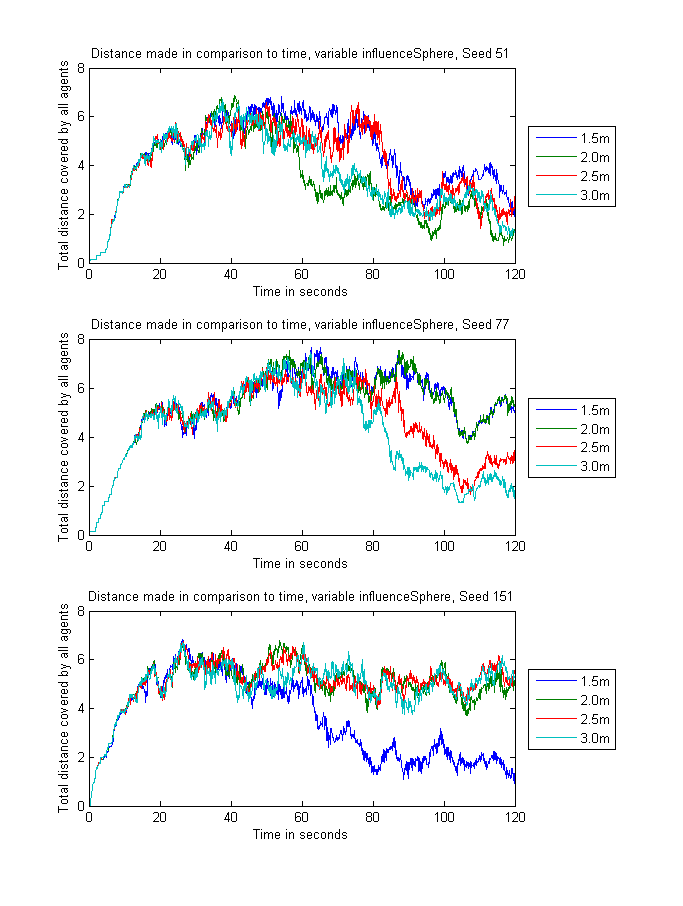
\includegraphics[width=0.80\textwidth]{../../code/sim/Width/ADistancesPerSeeds.png}
	\caption{This plot shows the total distance covered by all agents in the system for different influence sphere radii and seeds in dependence of the simulation time. This distance decreases rapidly when a jam starts. To investigate the radius' dependence on the total distance, the total plot was split up into three parts, each containing all simulations for one seed. Only these radii were varied in these simulations. One can see here that in seed 51, every simulation jammed independently of the radius. In seed 77, the larger radii jammed, on the other hand only the small radius crashed in seed 151.}
	\label{fig:SeedsOverview}
\end{figure}

To investigate this further, the plot was now split up into 3 subplots, one for each seed as figure \ref{fig:SeedsOverview} shows. Again, this seems to show some dependency as assumed in figure \ref{fig:SeedsColoured}, but this could also be coincidence.\\
Here, no dependency can be seen because with seed 51, every single simulation will cause jams. Seed 151 shows what one could expect to see: For a small influence sphere radius, a jam pops up. But seed 77 shows the exact opposite of this as here, the larger influence radii caused jams. So neither dependence nor tendency between influence sphere radius and total distance walked can be observed.

%Discussion
As already seen in chapter $hier verweis zur resultate-section von dieser serie einf�gen$, neither dependence nor tendency between influence sphere radius and total distance walked can be observed because there were opposing trends. Seed 151 showed what we expected to see: For a small influence radius, a jam popped up where for larger radii it didn't. On the other hand, seed 77 showed the exact opposite: only the large radii caused jams.\\
This leads us to think that coicidence played a main role here and shows us another thing: In our formulas weighing the influence of other agents on a specific agents, the weights are too big for very close agents in comparison to agents in a larger distance. This explains why larger radii didn't show the expected results: the additional influence of those agents was too little to matter. The assumption that out weighing function is not perfect can also be observed in any simulation: The agents walk straight forwards to each other for a long time and avoid each other only when they are very close to each other and not from a few meters ahead.
\label{ex3}

\subsubsection{Influence of the hallway width on the success of the simulation}
% Influence of the hallway width on the success of the simulation


\label{ex4}

\subsubsection{Simulating measurements of the main station Zurich}
% Simulating measurements of the main station Zurich

\noi The experiments were only analyzed visually by judging how well our model could cope with the given task and how it compared to the real observations. In figure \ref{fig:ex5picture}, one final situation for each run is given as an example.\\

\begin{figure}[h!]
	\centering
		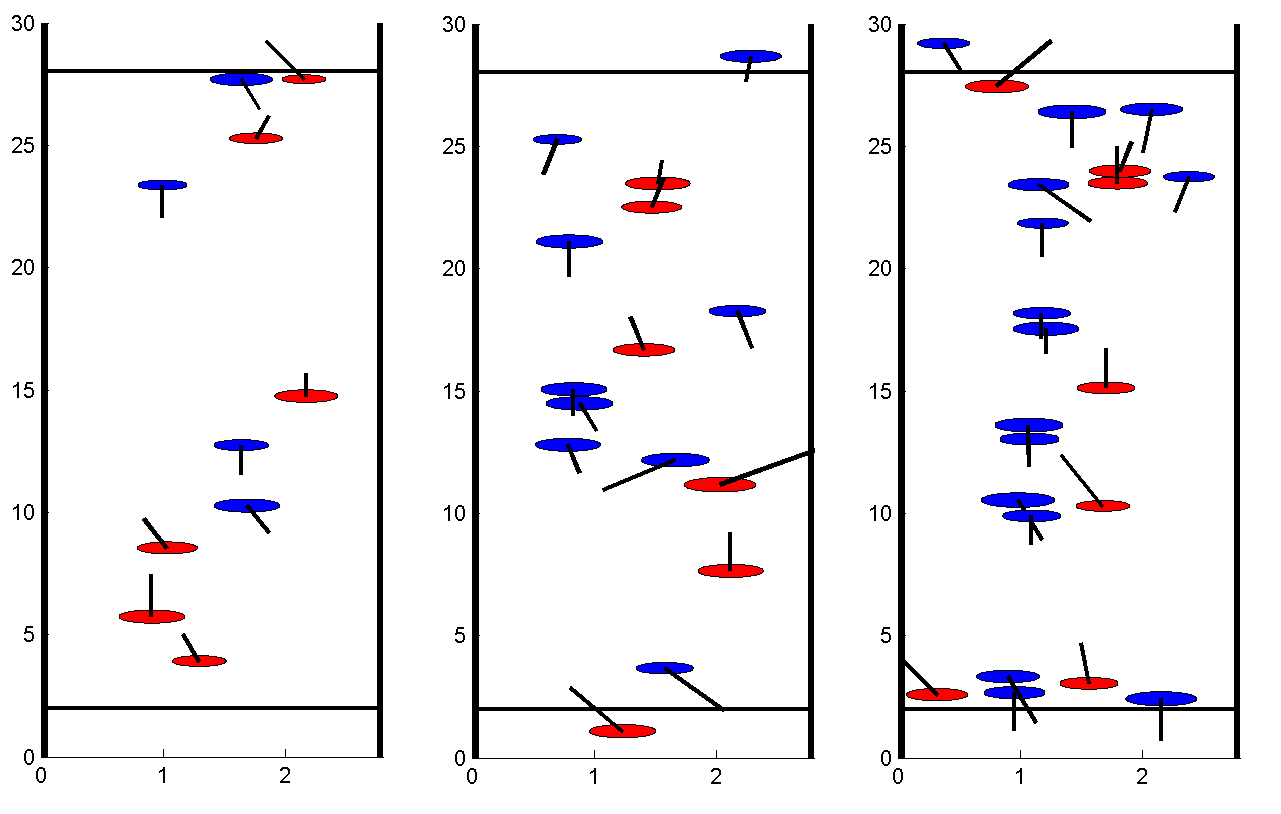
\includegraphics[width=0.90\textwidth]{pictures/ex5picture.png}
	\caption{Exemplary pictures for the simulation of the long narrow hallway in the Zurich main station. Red agents are walking up and blue down, the black line denotes the actual velocity vector with its angle and length. The left was done with flux densities of 0.12/0.17, the middle with 0.34/0.275 and the right with 0.6/0.5 after a simulation time of 180 seconds. In all investigated situations, the agents managed to cross the hallway without significant hindrance from other agents.}
	\label{fig:ex5picture}
\end{figure}

\noi For the first simulation series with a low people flux, the agents had no problems and could avoid collisions/walking into each other easily. This is in accordance with the observations.\\

\noi For the second simulation series with a medium people flux, the agents had little problems crossing the hallway. The stop-and-go of the observation was only rarely seen, suggesting that the logic behind our model is actually quite good.\\

\noi In the third simulation series with a high people flux, the agents had to stop sometimes while getting on the other side. But overall they could cope quite well with the task and the frequency of agents bumping into each other was quite slow and definitely in the same range as in real situations. Sometimes a small lane formation could be observed.\\

\noi We can say that our simulation worked well on the measured quantities. Of course, in reality, when jams start, there will be more side effects as people pushing, turning around, or trying to walk another way, but for a straightforward walk, our simulations mirrors the reality nicely.


\subsubsection{Simulation of a big inequality in the flux densities}
% Simulation of a big inequality in the flux densities

\begin{figure}[h!]
	\centering
		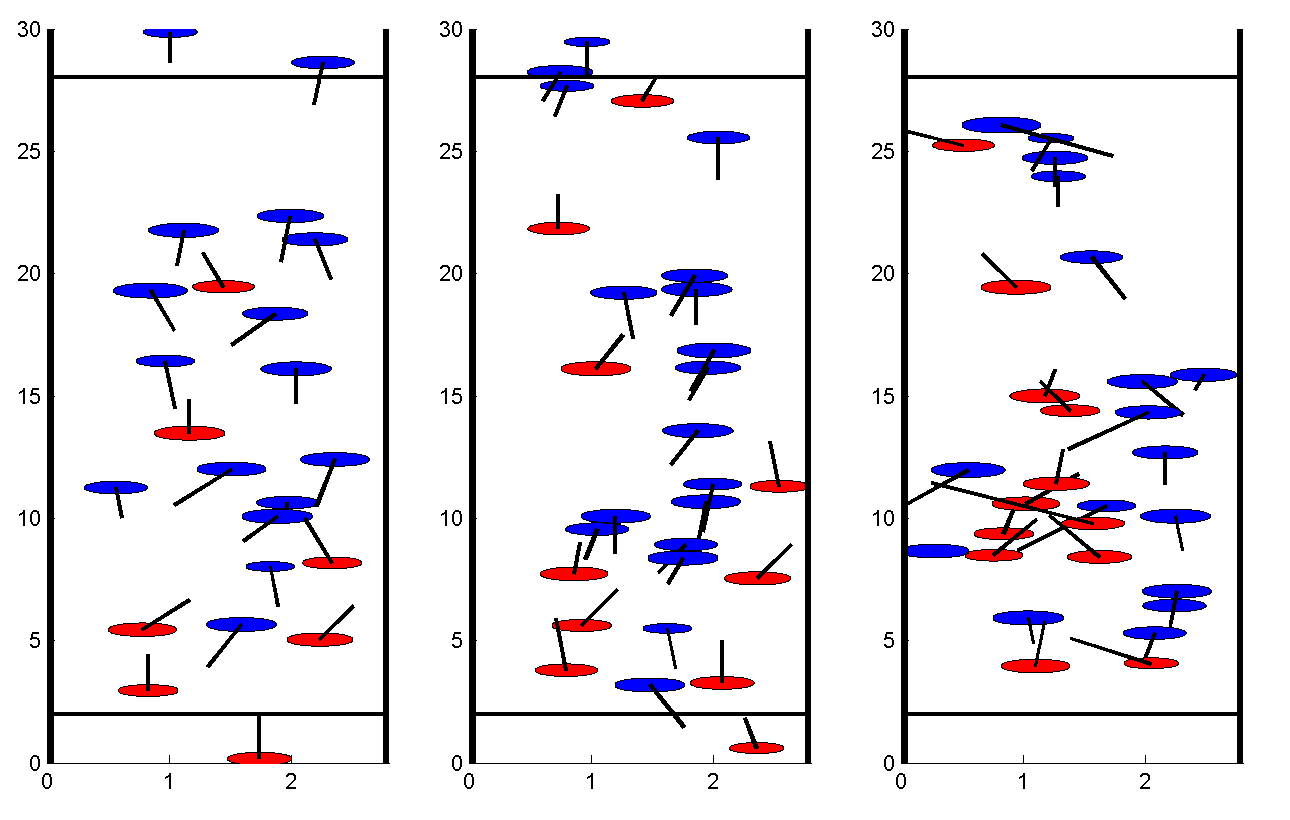
\includegraphics[width=0.85\textwidth]{pictures/ex6picture.png}
	\caption{Exemplary pictures for the simulation of the long narrow hallway in the Zurich main station with highly unbalanced flux densities. Red agents are walking up and blue down, the black line denotes the actual velocity vector with its angle and length. The one on the left was done with flux densities of 1.0/0.2, the one in the middle with 1.0/0.3 and the one on the right with 1.0/0.4 after a simulation time of 180 seconds. The red agents (minority) were wandering about quite strong and usually formed small lanes.}
	\label{fig:ex6picture}
\end{figure}

\noi The experiments were only analyzed visually by judging how well our model could cope with the given task. Some exemplary pictures are given in figure \ref{fig:ex6picture}.\\

\noi For the densities 0.2/1 used in the first series, the overall success was satisfying. The agents walking up (red, minority) were wandering about quite strong due to all the oncoming blue agents. But even though the blue outnumbered the red agents 1:4, the red agents stopped very rarely.\\

\noi In the case of the densities being 0.3/1, the results were quite similar with those obtained by 0.2/1. But the tendency for the red agents to walk in lanes or small groups increased clearly, probably because there are more red agents which are shuffled together by the big number of blue agents trying to stomp their way through.\\
\begin{figure}[h!]
	\centering
		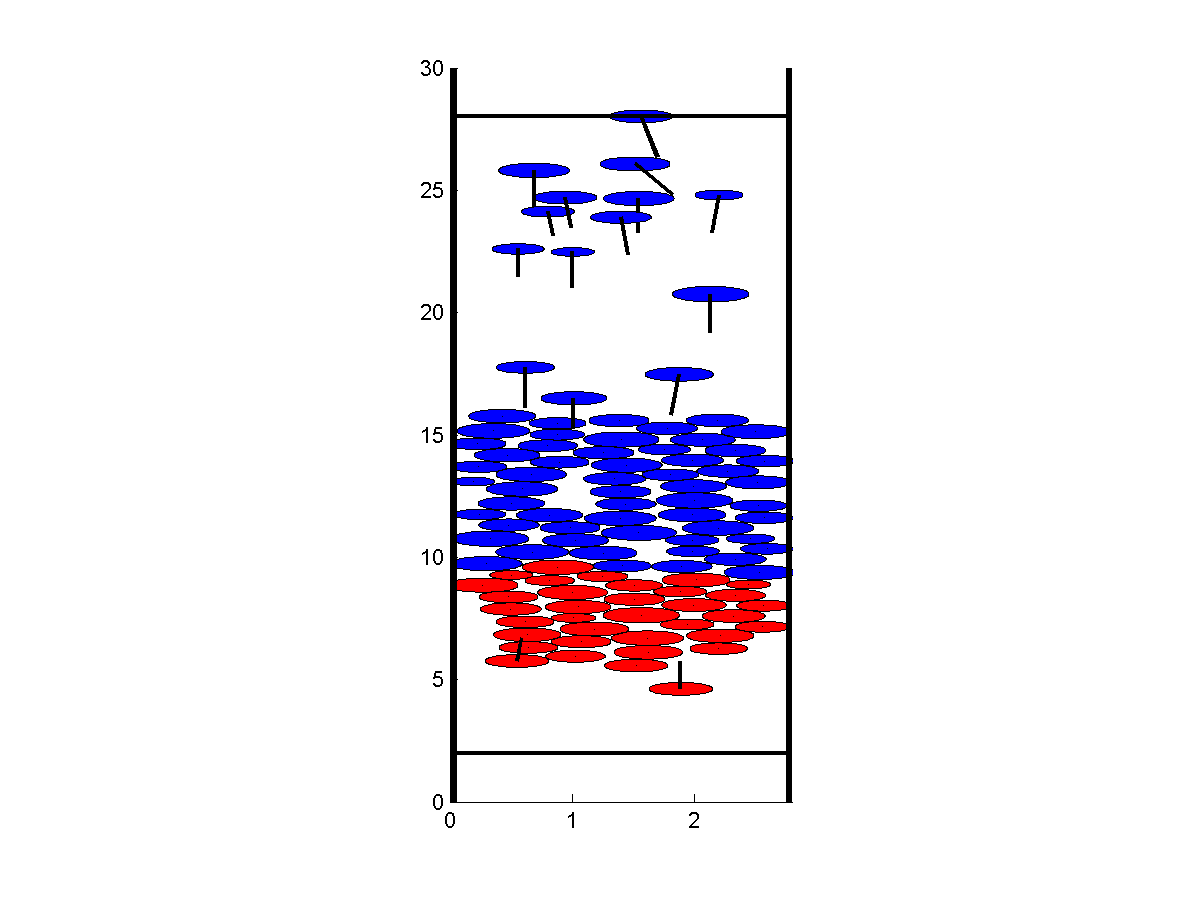
\includegraphics[width=0.90\textwidth]{pictures/up1down04seed51.png}
	\caption{Exemplary pictures for a massive jam in our model. Red agents are trying walking up and blue down, the black line denotes the actual velocity vector with its angle and length. Parameters were flux densities 0.4/1 with a seed of 51. Our model has no way to resolve a jam like that.}
	\label{fig:up1down03seed51}
\end{figure}

\noi For the last considered case, the simulation failed in one case after approximatly 140 seconds (seed 51). The situation after 180 seconds is given in figure \ref{fig:up1down03seed51} as a classical example of how a jam looks like in our model. Before that and in the other two simulations, the red agents formed lanes and little groups very frequently as a way to not always get tossed over the whole width.\\
But the failure suggests that we reached about the limit which can be modelled with our simulation.\\

\noi To sum up, we can say that what we expected could be observed. Anyone who ever went against the tide, for example when people debark a train or bus, knows that advancement is hard to reach. This effect of slowing down and flocking together with other people who try to walk the same way popped up nicely.\\


\subsection{Discussion}
\subsubsection{Simulations}
Overall, we were quite pleased with the results we got from our simulations as they mostly fulfilled our expectations. We could underscore the importance of the choice of a good set of parameters for our model to succeed. It is also possible, as in the case of \texttt{DISPFACTOR}, that parameter changes can change the result drastically.\\
To address the question whether our model is a good description of the reality even if it cannot decide on itself whether it should start something like a cooperative mode including lane formation or adapt an egoistic approach, we would like to state that the model is only as intelligent as the one who uses it. We leave it to the user of the simulation to set reasonable (and therefore also realistic) values for the global parameters which should match the situation one would like to research.\\

\noi The main simulations concerning the modelling of an actual situation was very satisfying as it performed at least as good as reality. A criticism onto our implementation of the main station in Zurich could be that the flux of people arriving is always kept constant. People familiar with the main station in Zurich would know that there is a pedestrian traffic light just in front of the Burger King, therefore the simulation should probably be adapted to allowing intermittent people spawning with different people flux densities just after the red or green light at the traffic light.\\

\noi It should be highlighted that we saw a big overall performance improvement once we introduced the preference for lane formation. This can be interpreted as implementing a social norm which states that one should back down a little bit from the egoistic main goal of crossing as fast as possible but work together in order to get an acceptable result for everyone. Also, it is similar to the phenomenon sometimes observed that people have the tendency to walk on the right hand side of their walking direction, used to this by traffic.\\

\subsubsection{Discussion on various implementational issues}
As we created and implemented our model from scratch, there are obviously some undealt issues that would need refinement if one wants an even better performance of the simulation as such.\\

\begin{figure}[h!]
	\centering
		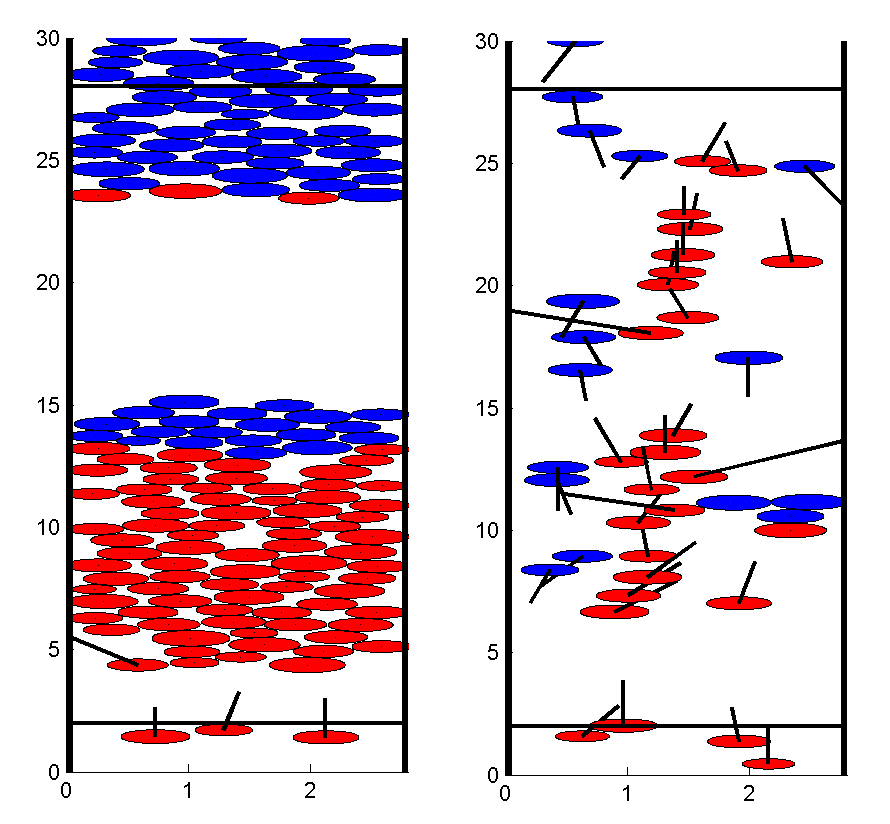
\includegraphics[width=0.90\textwidth]{pictures/exFails}
	\caption{Graphical examples of instructive failures. Graphs were taken from the simulation series to test \texttt{DISPERSIONFACTOR}. In the left graph, we have in the top region of the hallway the unrealistic situation where three agents block the whole hallway. On the right, the earliest stage of a jam is visible with the three blue and one red agent standing in the middle at the right wall. This situation won't resolve and so, a jam will start because agents walking into them from behind will get stuck too.}
	\label{fig:exFails}
\end{figure}

\noi Probably the most important issue of all would be the need of implementing a smarter way to resolve standoffs or detect them earlier. We reckon that a good implementation of this should prove to be rather difficult as one has to distinguish between various cases with various ways to resolve them. This is visualized in figure \ref{fig:exFails} in the right graph. As soon as two (or more) agents totally immobilize each other, they are prone to form a jam.\\
One would probably have to introduce walking backwards to resolve these situations. The effect of not being able to walk backwards is given in figure \ref{fig:exFails} in the left graph on the top in a very instructive way. Three red agents were able to totally freeze the simulation at the top, something that would never happen in reality.\\
Another advantage of a good implementation would be that the runtime on the machine would not explode as it does with the current implementation as soon as a jam has formed. This is rooted in the consideration that all agents within a certain radius shall be considered. Then the logical routine would do calculations over a lot of other agents, even though the agent will not be able to move anyway as he is stuck in a jam.\\

\noi We used two different axis, a $x$- and a $\varphi$-axis as we thought this would make it significantly easier to model various aspects without the trouble of doing the transformation on paper and only use the $\varphi$-axis all the way. Also all angular values had to be discretized to their closest values the $\varphi$-axis has, which was done with the function \textit{closest.m}. This works fine as long as the simulation runs smoothly, but as soon as a jam was formed, the number of calls of \textit{closest.m} exploded. In one case, it was called over 2 million times for 1200 iteration steps in a simulation that had a matlab runtime of about 2 hours (with 4 Matlab instances running parallel).\\

\noi It rarely happens during a simulation that an agent is in an impossible position. This is determined in the collision detection because the first of all calculated points is the position the agent stands on before moving. This was easier to implement and probably not significantly worse in system runtime than excluding it. In rare occasions, the collision detection determines that the agent could not stand at its actual position. We think that this happens due to some small roundoff errors or other computational mistakes.\\
If the agent is at an impossible position, its position would freeze and cause everything around him not to work properly anymore. We could not think of an effective algorithm to resolve these conflicts because they would probably involve setting back the simulation by some iteration steps, so we decided to simply delete such an agent.\\
We knew that it was not an elegant solution but could settle on the argument that the simulation would otherwise crash. And as the frequency of this occurrence is really small, we also thought that the number of disappearing agents could be neglected. For long simulations, this may not hold true any longer.\\

It is worth mentioning that an optimization of all the global parameters is quite difficult as they are anything but independent of each other. Therefore we settled on parameters that seemed to work quite well without an extensive testing.


